%% This is an example first chapter.  You should put chapter/appendix that you
%% write into a separate file, and add a line \include{yourfilename} to
%% main.tex, where `yourfilename.tex' is the name of the chapter/appendix file.
%% You can process specific files by typing their names in at the 
%% \files=
%% prompt when you run the file main.tex through LaTeX.

\singlespacing{

\chapter{Introduction}

A moonshot goal of digital fabrication is the bottom up programmable assembly of meter scale objects with nanometer scale precision.  With this technology, we could design materials with exotic physical properties and radically transform the way we make almost anything.  We believe this is possible by constructing nanoscale assemblers that work together to precisely control and place raw material feedstock.  Though it sounds like science fiction, biology has demonstrated that this is possible.  Data encoded in DNA can be executed like a computer program to build an immense assortment of molecular-scale machines, which together, coordinate the higher level structure and functions of an organism.
\\

Other parallels between biological assembly and our proposed system are the discretization of a relatively small number of different feedstocks and parallelization of assembly.  The protein machinery of biology is made primarily from the same basis set of 20 amino acids, yet proteins display a wide variety of functions and morphologies to carry out the many tasks of the cell in parallel.  Similarly, the material feedstock of the nano-assemblers consists of a finite set of part types, called "digital materials".  These digital materials are joined together in various patterns to produce diverse, functional structures.  Since construction takes place one nano-brick at a time, many assemblers would need to work in parallel to build structures of any significant size.  If the assemblers are designed in such a way that they can be constructed from their own feedstock, assemblers can build more assemblers and the rate of assembly scales exponentially.
\\

\begin{figure}
  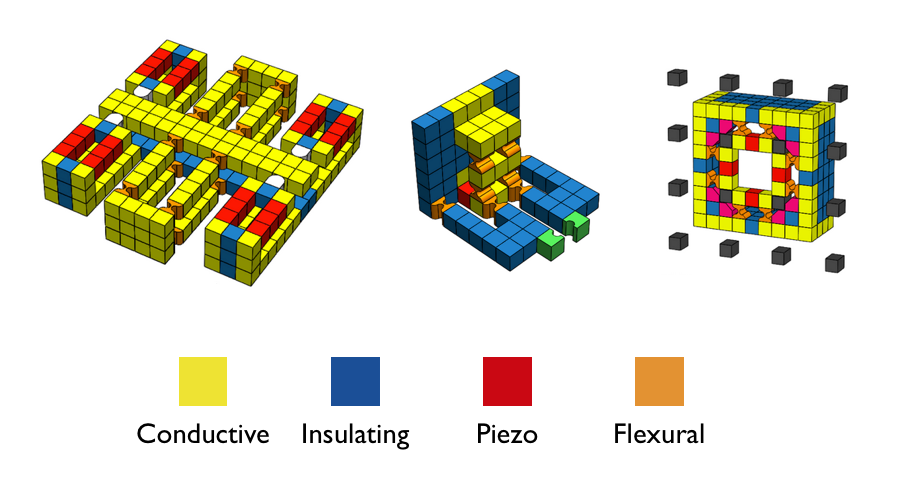
\includegraphics[width=\linewidth]{willMockups.png}
  \caption{Design mock-ups of assembler components made from digital materials by Will Langford.  From left to right: a linear actuator, a part gripping mechanism, a clamping mechanism.  None of these designs has been evaluated in simulation.}
  \label{fig:willMockups}
\end{figure}
The nano-assembly I've described will look very different from the way we make things today, and opposes many of the assumptions baked into traditional Computer Aided Design (CAD),  Computer Aided Manufacturing (CAM), and robotics.  This assembly strategy follows from an existing line of research called "digital assembly", where discrete parts are assembled on a regular, periodic lattice.  Mechanical systems are built with discrete modules of rigid and flexural components, and electronics and controls are distributed spatially across a machine (Fig \ref{fig:willMockups}).  Large structures appear to be "living" in the sense that their surface is teeming with nano-robots, detecting and correcting errors and performing other functions.  The environment is highly structured, allowing locomotion systems to position themselves globally by counting local movements across a lattice.  Machines receive instructions from their environment to coordinate various tasks.
\\

\section{Proposed Work}

I propose to build a design/simulation environment for digital materials based on realistic materials and physics, so that structures designed within this virtual environment may be physically realized one day.  I will use this virtual sandbox to design basic functional elements needed for the eventual goal of building a physically realizable assembler capable of self-replication.  Some elements of interest include mechanisms for grasping and moving parts in the assembler's environment, locomotion systems, information storage and retrieval, amplification, and digital logic.

\subsection{Part Types}

A major part of the initial phase of this project involves a literature review of research spanning biology, cellular automata, modular robotics, and materials science to pick the basis set of parts, their length scale, and a scheme for joining them together.  Initial sketches of the part types include rigid, flexure, piezo, conductive, insulating, capacitive, and resistive and scales ranging from $\mu$M to mm on a side.  The parts may become more complex for larger scales of bricks (transistors/logic gates).

\subsection{CAD Interface}

%\begin{figure}
%  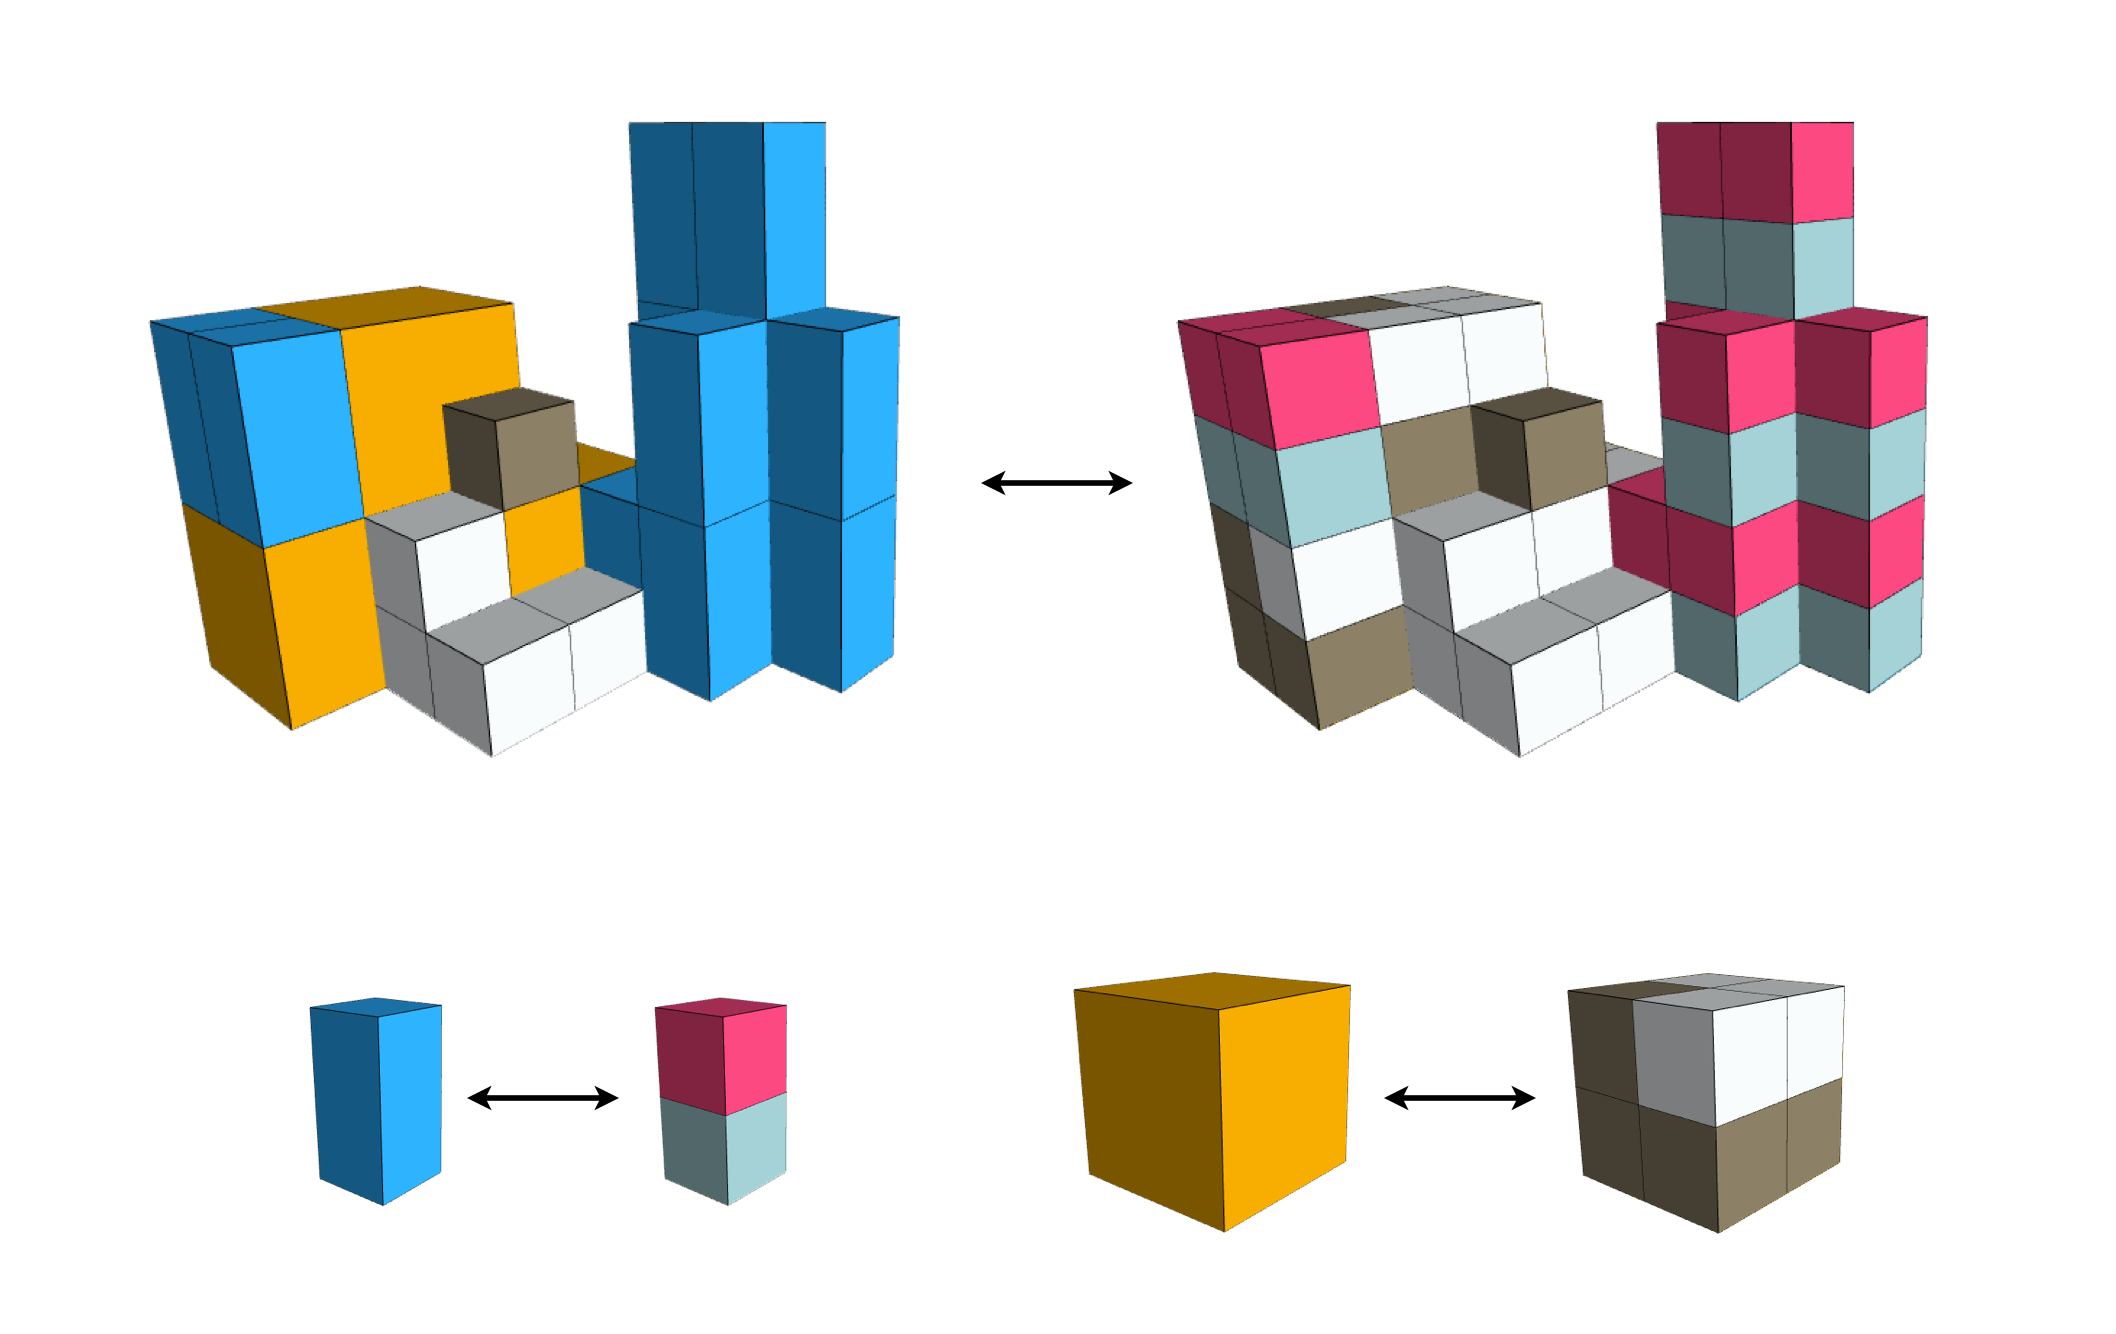
\includegraphics[width=\linewidth]{hierarchicalDecomp.png}
%  \caption{Hierarchical decomposition of lattice assembly. All hierarchical components are parametrically linked to a hierarchical material definition.}
%  \label{fig:hierarchicalDecomp}
%\end{figure}

Borrowing some classes and frameworks I've started in DMDesign, I will create a new project for the work spawned from this thesis.  All geometry will be assumed to fit on a regular cubic lattice, though flexural deformations may allow for off-grid motions.  Geometry will be represented in a hierarchical fashion (as is the case in DMDesign), where subassemblies of parts can be defined and patterned across a design, and all instances of a subassembly are linked parametrically to the same definition.

%\begin{figure}
%  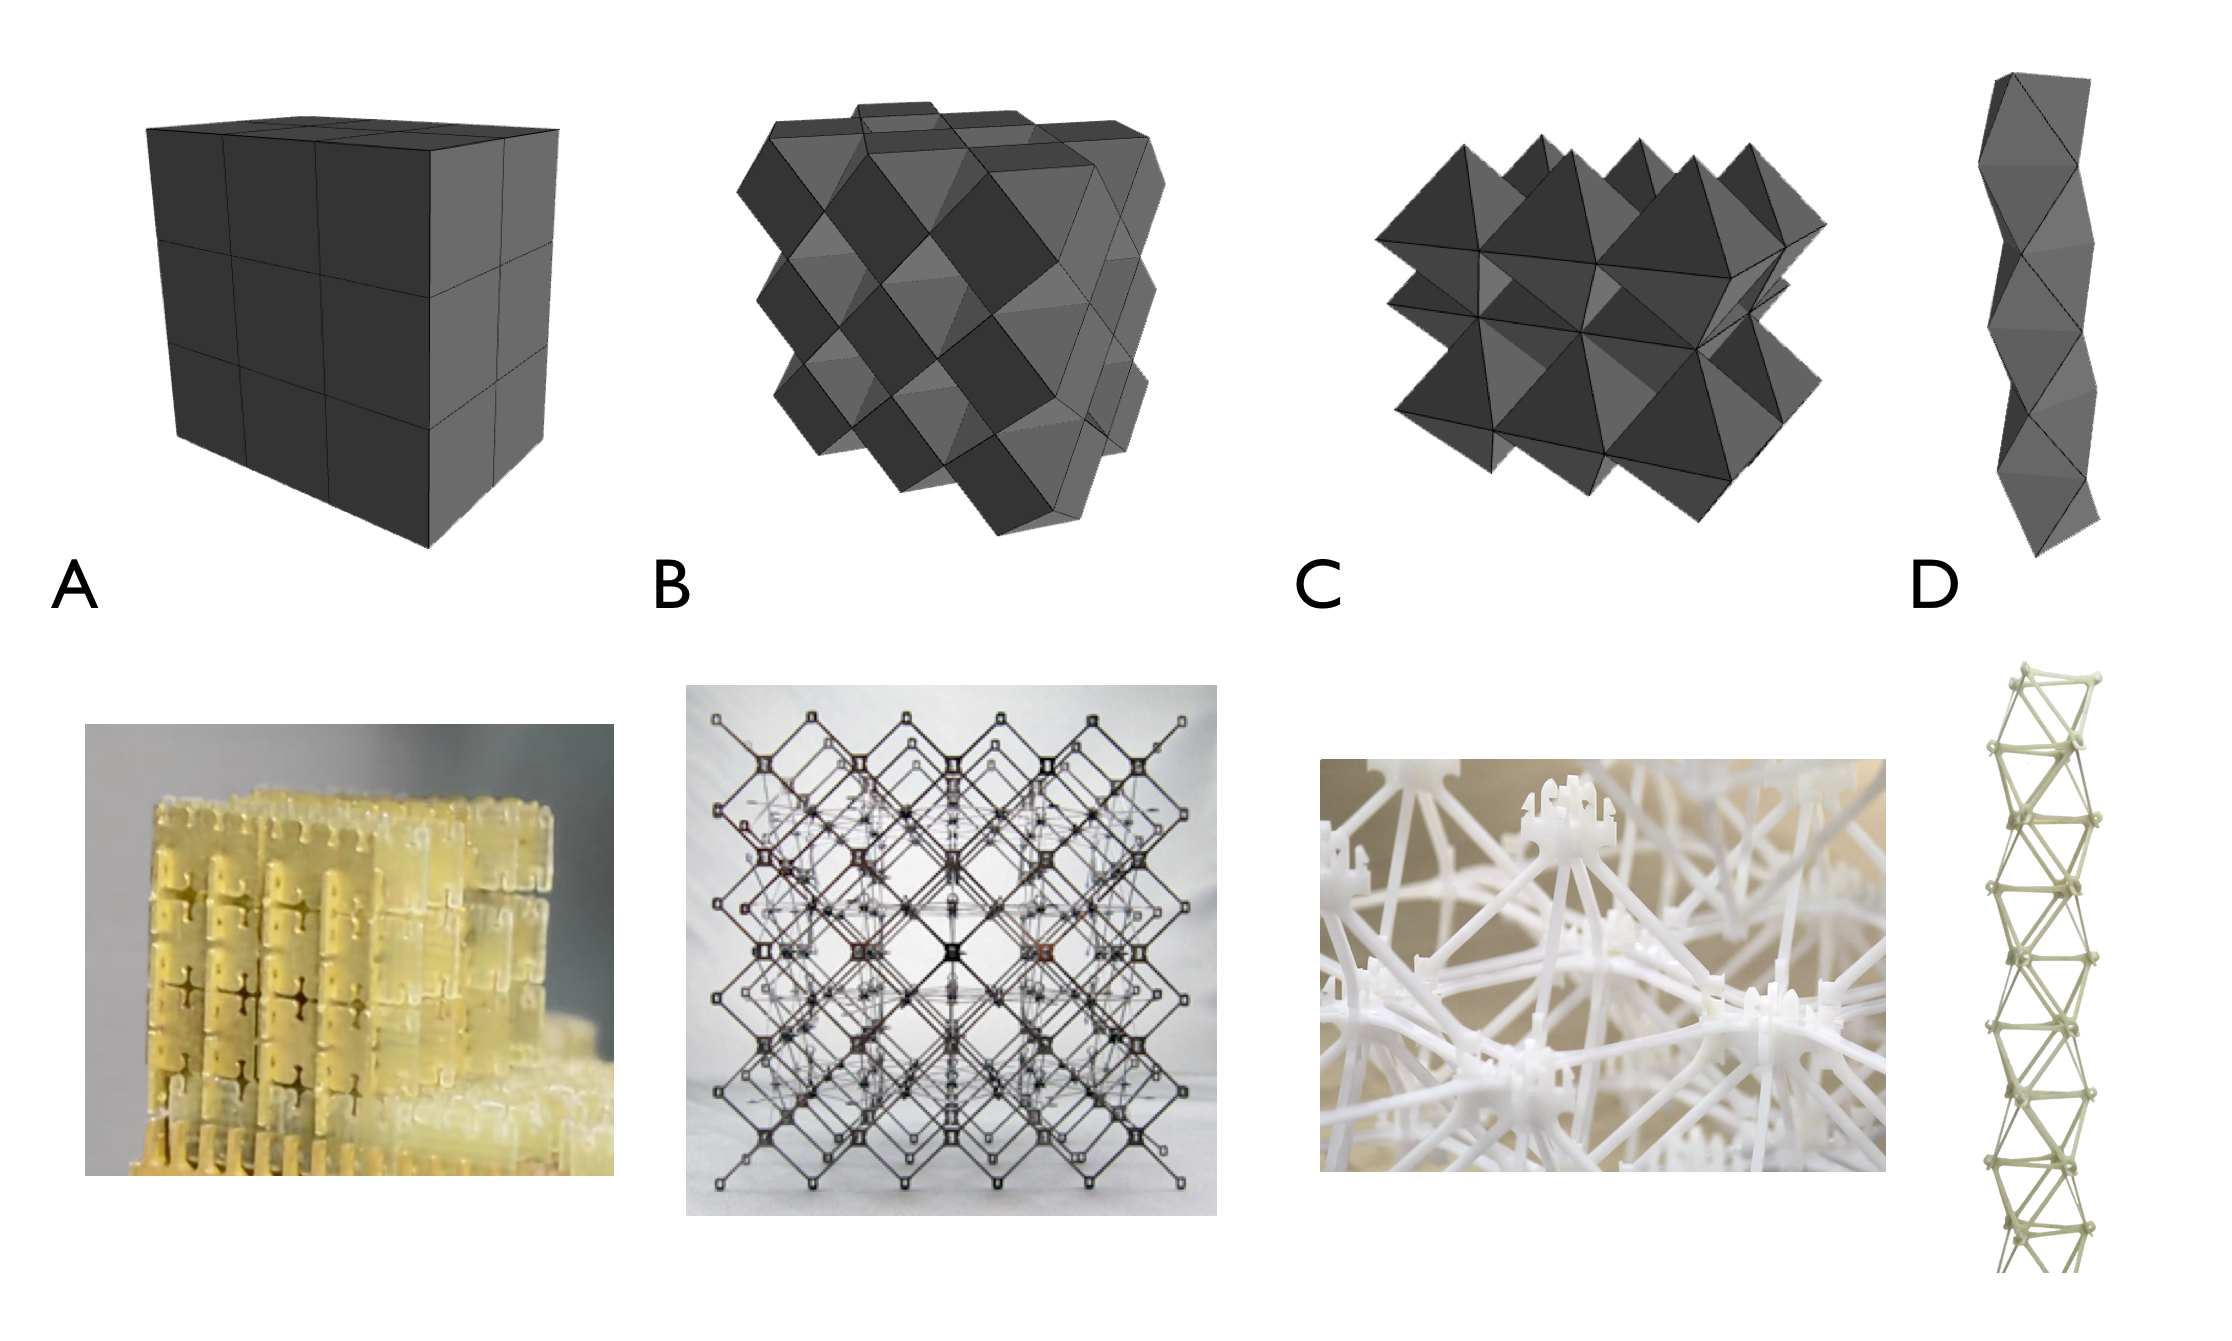
\includegraphics[width=\linewidth]{latticeVirtualRealComp.png}
%  \caption{Comparison of virtual lattice types with their real world counterparts.}
%  \label{fig: latticeVirtualRealComp}
%\end{figure}

%\begin{figure}
%  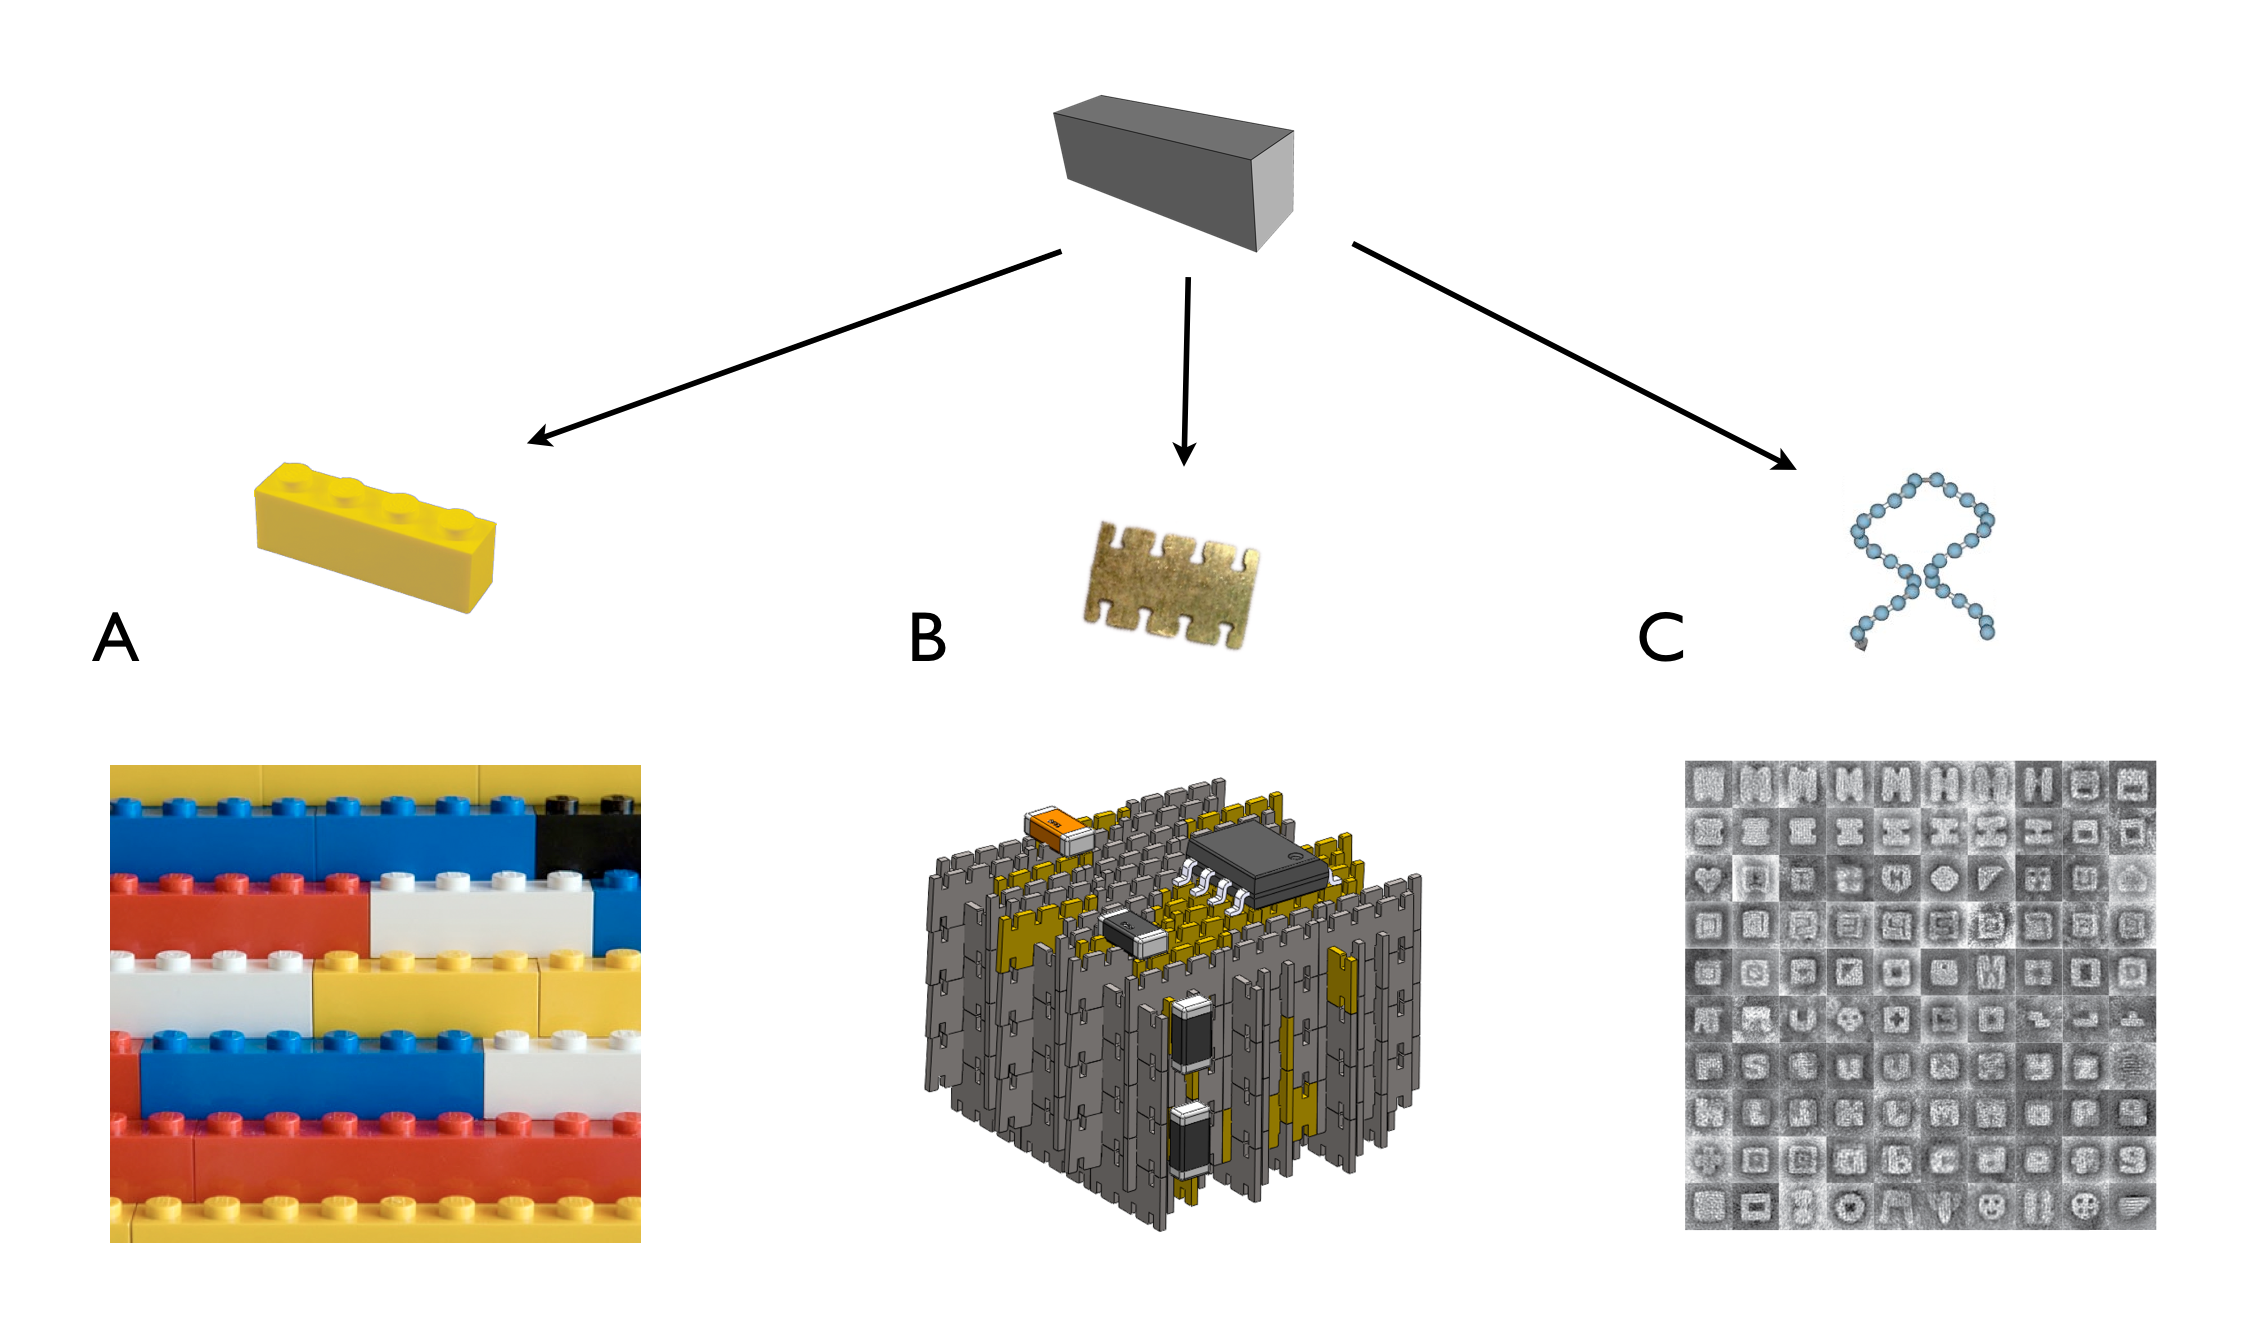
\includegraphics[width=\linewidth]{partAbstraction.png}
%  \caption{Part abstraction from lattice primitive.}
%  \label{fig: partAbstraction}
%\end{figure}

\subsection{Simulation Engine}

Dynamic simulation occurs at the granularity of the cell by modeling only local interactions between a cell and its immediate neighbors.  This way, as an assembly is designed through the CAD interface, its corresponding simulation model is constructed at the same time.  I hope that by implementing a local-only mode of simulation, I will be able to reuse the same connectivity model for both mechanical and electronic simulation, and cut down on computational costs.
\\

Locating parts on regularly spaced intervals on a lattice allows for computational shortcuts in simulation.  Depending on the nature of the mechanical and electronic simulation, I may be able to use a hash table to increase performance\cite{Gosper1984}, especially for repeating hierarchical structures within a model.  Previous work has adapted the hashlife algorithm for kinematic systems of cellular automata\cite{Stevens2010}.  I will surely need to spend some more time looking into this literature before implementing it in my own system.
\\

Additionally, I will need to implement some kind of collision detection for this system.  Due to the prevalence of gaming, there are an assortment of published algorithms to speed up  collision detection over the obvious naive approaches.  Many physics engines rely on a boundary representation of an object to detect collision with other boundaries - if objects are moving too quickly this can lead to unexpected results.  The voxels in my geometry will together define a volume of space, and the cells forming the boundary of this volume are known; I will leverage this to cut down the computational costs of collision modeling in my simulations.

\subsection{Approach}

The proposed digital materials sandbox will be built in Javascript using the following dependencies (more may be added):
\begin{itemize}
\setlength\itemsep{0em}
\item \href{http://threejs.org/}{Three.js} is a library that makes WebGL easy to use without sacrificing much in performance
\item \href{http://requirejs.org/}{RequireJS} is a framework for asynchronously loading javascript modules and dependencies
\item \href{http://backbonejs.org/}{Backbone.js} is a framework for managing UI events and giving structure to an interactive application
\item \href{https://jquery.com/}{JQuery} is a library that simplifies interactions with HTML and helps maintain cross-browser support
\item \href{http://underscorejs.org/}{Underscore} is a library with lots of useful functions for dealing with arrays and javascript objects
\end{itemize}

I know I will take some performance hit writing this application in JavaScript as opposed to a strongly-typed language like C running natively, but for this first implementation it makes sense to do start with a programming environment that I can rapidly develop in and experiment with.  If it turns out that I need to design very large structures in CAD or performance is getting in the way, I will consider porting the codebase into a compiled format.  With some optimization of the rendering, it is possible to render 100-200k voxels on the screen at 30fps in Three.js, it is unclear at this time exactly how costly the simulation will be.
\\

Aside from my own familiarity with web development, I'm interested in using HTML5/ Javascript for this application because it allows easier access to the code than any other platform.  Though user studies are not a component of this work, there is a long history of communities of users building things in these types of sandbox environments that surpass anything the developers were able to imagine.  There is a lot of talent beyond the immediate neighborhood of CBA, and I'd like to try to make this codebase as available as possible for anyone interested in exploring this new way of making things.

%\subsection{Assembly}
%
%\begin{figure}
%  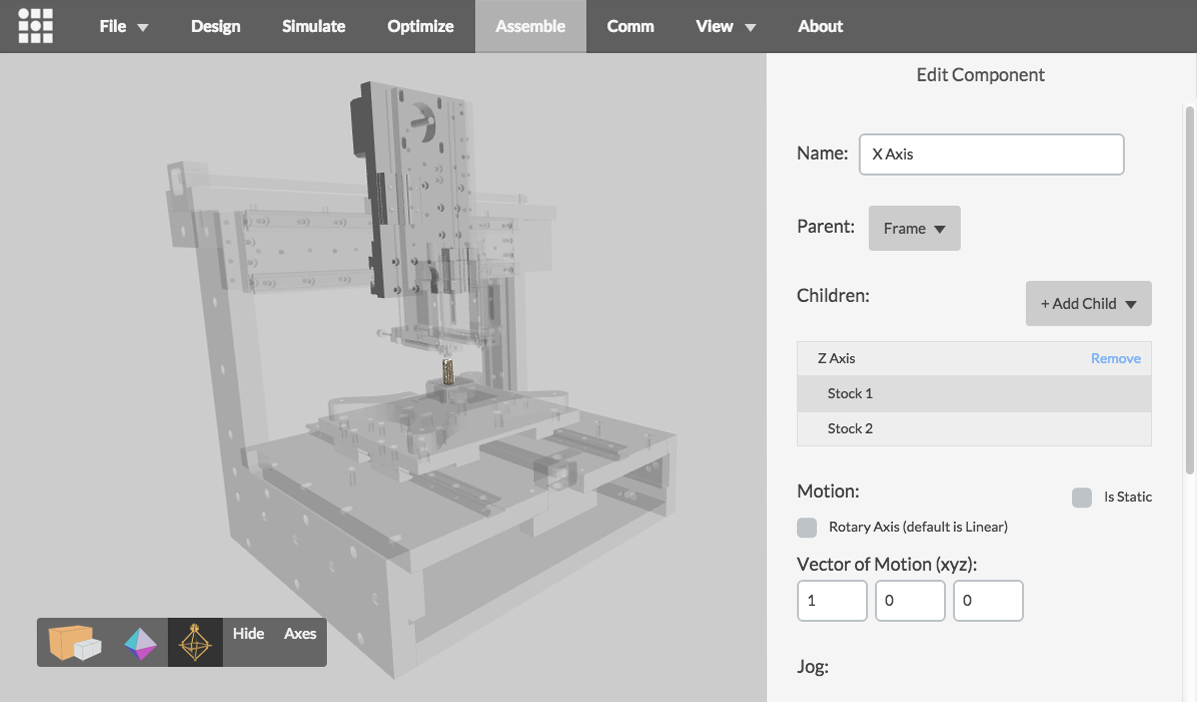
\includegraphics[width=\linewidth]{assemblerSetup1.png}
%  \caption{Screenshot of current assembler config GUI.}
%  \label{fig: assembleSetup1}
%\end{figure}
%
%\begin{figure}
%  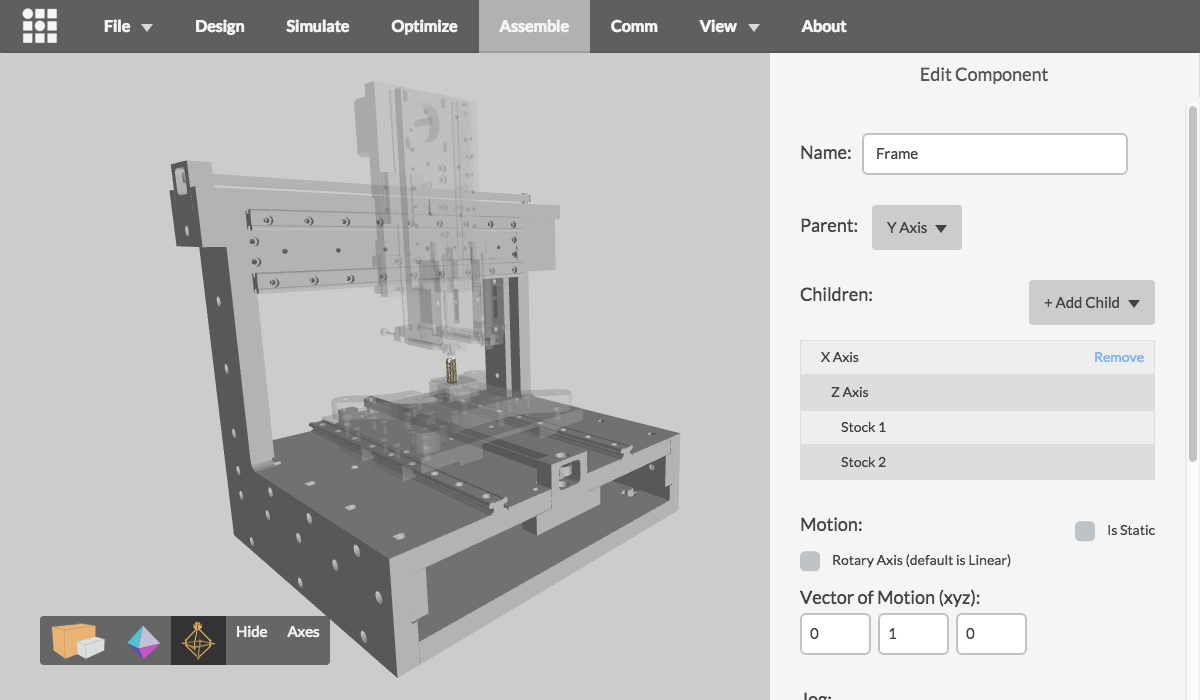
\includegraphics[width=\linewidth]{assemblerSetup2.png}
%  \caption{Screenshot of current assembler config GUI.}
%  \label{fig: assembleSetup2}
%\end{figure}
%
%urdf, tree description for abstraction
%calculate reverse kinematics
%abstraction of strategies and assemblers/low level operation

%\subsection{GUI}
%
%\begin{figure}
%  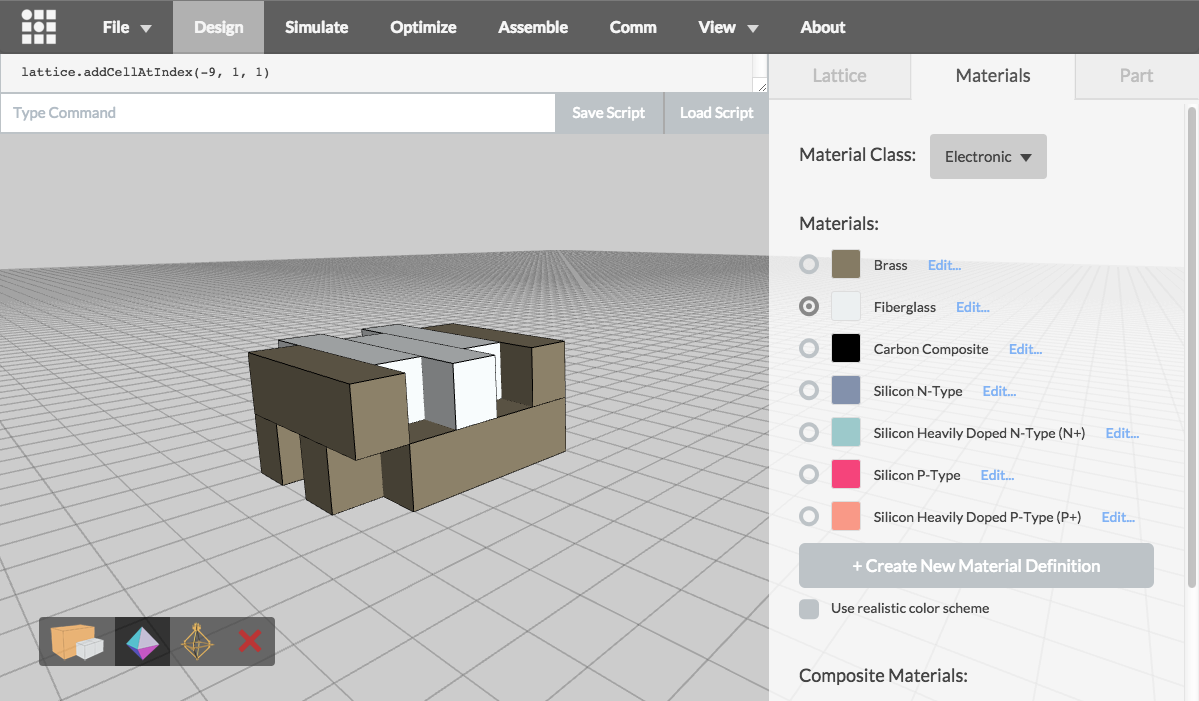
\includegraphics[width=\linewidth]{designGUI.png}
%  \caption{Screenshot of current design GUI.}
%  \label{fig: designGUI}
%\end{figure}
%
%\begin{figure}
%  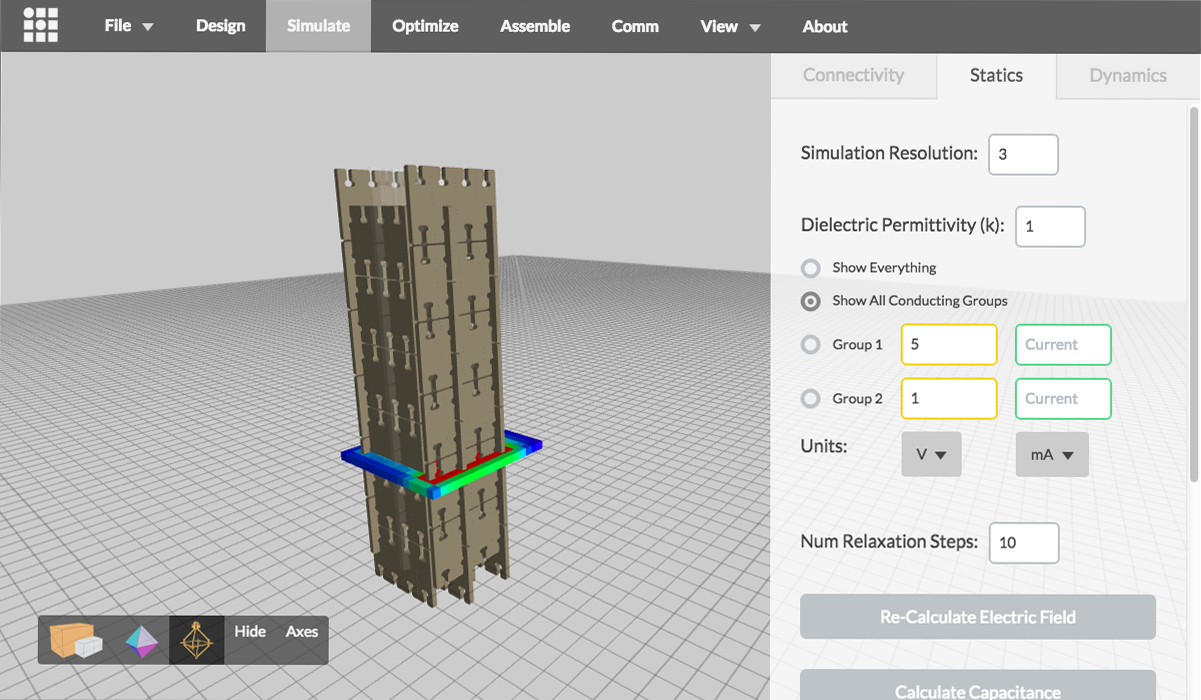
\includegraphics[width=\linewidth]{simGUI.png}
%  \caption{Screenshot of current simulation GUI.}
%  \label{fig: simGUI}
%\end{figure}
%
%\begin{figure}
%  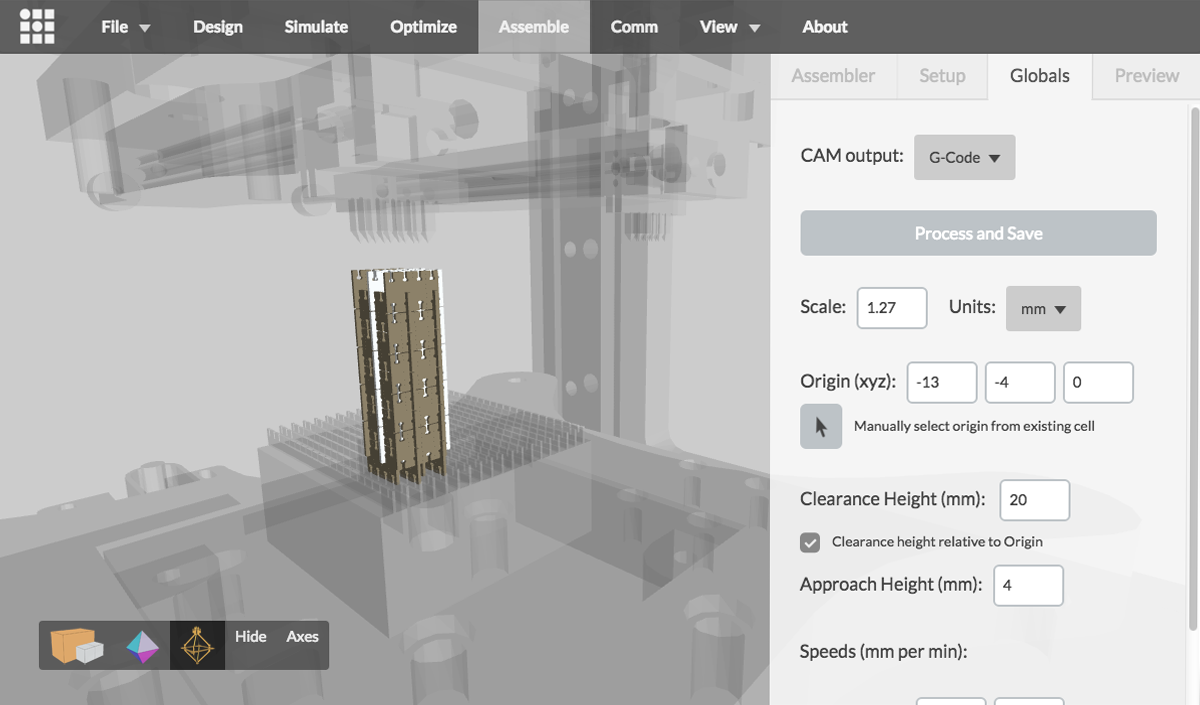
\includegraphics[width=\linewidth]{assembleGUI.png}
%  \caption{Screenshot of current assemble GUI.}
%  \label{fig: assembleGUI}
%\end{figure}
%
%javascript, etc, etc

%\subsection{API}
%
%Lattice, Cell, Material, CompositeMaterial classes.
%
%\begin{figure}
%  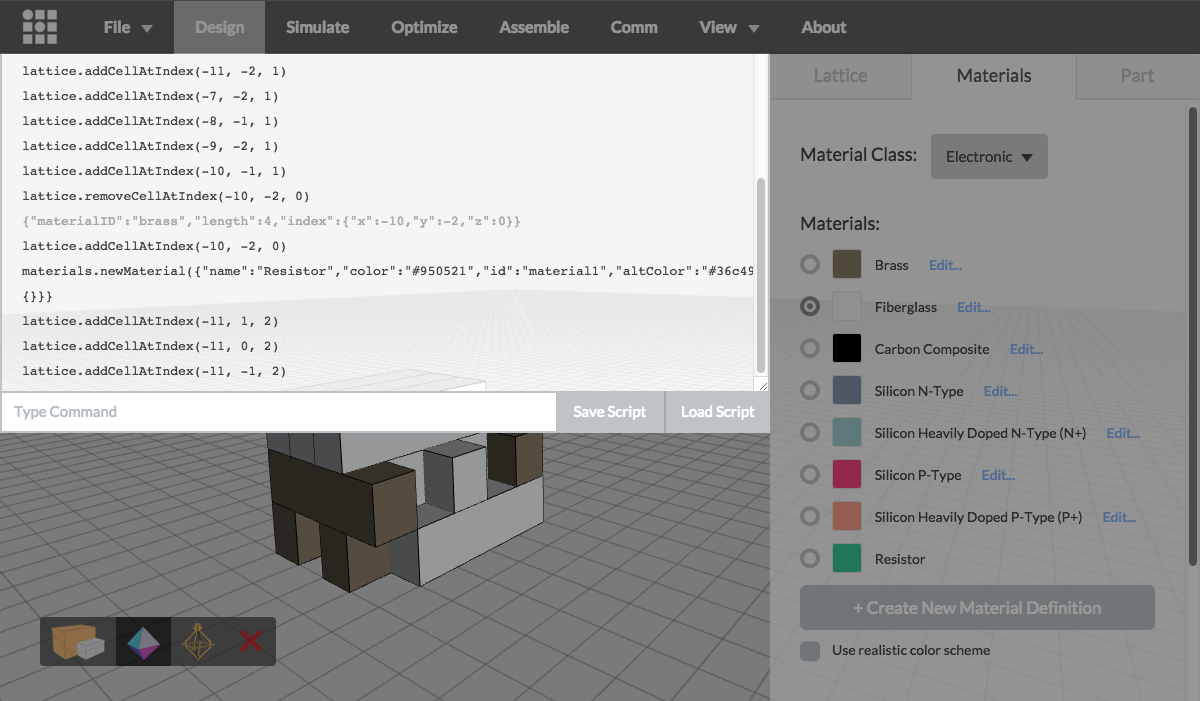
\includegraphics[width=\linewidth]{scriptGUI.png}
%  \caption{Screenshot of current script GUI for API with scripting console highlighted.}
%  \label{fig: scriptGUI}
%\end{figure}
%
%asdfdsf

\section{Contribution}

As outlined in previous sections, the main contribution of this work is to create a design/simulation environment where anyone can start to explore the rich design space around digital materials in a physically realistic way.  This work will inform future trajectories in CBA research and in the broader field of programmable materials, modular robotics, and digital fabrication.  This work is not intended to result in a manual outlining all the necessary components for self-replication based on current technology, but rather as an sandbox for exploring self-assembling systems based on the foundations of engineering and materials science rather than biology.

\section{Evaluation}

Once the CAD/simulation environment is set up, I will design several functional objects within it and evaluate their function both quantitatively and qualitatively.  Some objects that would be especially interesting include:
\begin{description}
\setlength\itemsep{0em}
\item[] locomotion systems
\item[] end effectors (gripping mechanisms, part manipulation)
\item[] information storage and retrieval
\item[] amplification of motion and signals
\item[] digital logic
\end{description}
Qualitative assessment includes evaluation of success or failure of the intended function (can a gripping mechanism grip a part), and quantitative assessment includes calculations of performance (gripping strength, speed of locomotion, volume required to implement various types of digital logic, speed of memory access, etc).

\section{Resources Required}

The majority of the work involved in this thesis will happen in the computer and require no material resources.  If required, I will use CBA's cluster for highly parallel computational operations.  Fabrication of assemblers and parts to be used in the digital assembler workflows should be considered outside the scope of material resources required by this thesis, and will be supplied by CBA.

\section{Schedule}

\begin{description}
  \item[11/6/15]\tabto{1.5cm}Proposal Due
  \item[11/9/15]\tabto{1.5cm}Crit Day Presentation
  \item[11/15]\tabto{1.5cm}Design and assembly workflow for digital materials is in a working state.  I will use elements of the classes and framework developed in that project to begin a new project specifically for the completion of the thesis.  This new project will only be concerned with the design and simulation of multimaterial assemblies on a cubic lattice (for simplicity).  Finish CAD interface.
  \item[12/15]\tabto{1.5cm}Hello world of basic CA behind the electronic/mechanical simulation.  Not worrying about efficiency at this point, get cells moving and communicating.  Start making decisions about scale and part types, num materials, geometry, allowed interactions, interfaces.
  \item[1/15]\tabto{1.5cm}Build out main components of simulation engine.
  \item[2/15]\tabto{1.5cm}Collision detection strategies, unconnected modules should be able to interact with each other
  \item[3/15]\tabto{1.5cm}Refinement and optimization of simulation engine
  \item[4/15]\tabto{1.5cm}Performance optimization and design studies
  \item[5/15]\tabto{1.5cm}Design studies and writeup
  \item[6/6]\tabto{1.5cm}Thesis Due
\end{description}

}
